\documentclass[tikz,border=2pt]{standalone}
\usepackage{amsmath}
\usetikzlibrary{arrows.meta}
\begin{document}
% At i = 0.04 the four rates of one interest basis on a number line:
% d = 0.038462 < delta = 0.039221 < i^(12) = 0.039285 < i = 0.04; i^(m) decreases to delta as m grows.
% x coordinate = 3.5 cm per 0.001, measured from 0.038.
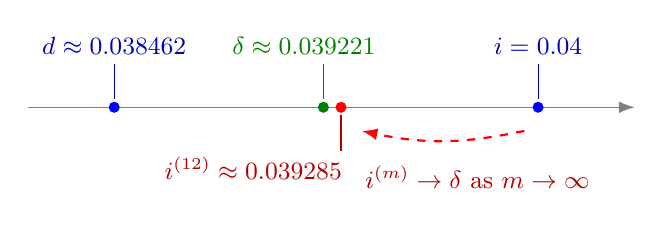
\begin{tikzpicture}[font=\small, >={Latex[length=2mm]}, x=3.5cm, y=1cm]
  \draw[gray, ->] (0.15,0) -- (2.35,0);
  % rates
  \foreach \x/\c in {0.462/blue, 1.221/green!50!black, 1.285/red, 2.0/blue} {
    \fill[\c] (\x,0) circle (2pt);
  }
  \draw[blue!70!black, thin] (0.462,0.1) -- (0.462,0.55);
  \node[blue!70!black, anchor=south] at (0.462,0.55) {$d\approx0.038462$};
  \draw[green!50!black, thin] (1.221,0.1) -- (1.221,0.55);
  \node[green!50!black, anchor=south] at (1.15,0.55) {$\delta\approx0.039221$};
  \draw[red!70!black, thin] (1.285,-0.1) -- (1.285,-0.55);
  \node[red!70!black, anchor=north east, inner sep=2pt] at (1.31,-0.55) {$i^{(12)}\approx0.039285$};
  \draw[blue!70!black, thin] (2.0,0.1) -- (2.0,0.55);
  \node[blue!70!black, anchor=south] at (2.0,0.55) {$i=0.04$};
  % i^(m) -> delta
  \draw[->, red, thick, dashed] (1.95,-0.3) to[bend left=12] (1.36,-0.3);
  \node[red!70!black, anchor=north] at (1.78,-0.62) {$i^{(m)}\to\delta$ as $m\to\infty$};
\end{tikzpicture}
\end{document}
